%%%%%%%%%%%%%%%%%%%%%%%%%%%%%%%%%%%%%%%%%%%%%%%%%%%%%%%%%%%%%%%%%%%%%%%%%%%%%%%%
%2345678901234567890123456789012345678901234567890123456789012345678901234567890
%        1         2         3         4         5         6         7         8

\documentclass[letterpaper, 10 pt, conference]{ieeeconf}  % Comment this line out
                                                          % if you need a4paper
%\documentclass[a4paper, 10pt, conference]{ieeeconf}      % Use this line for a4
                                                          % paper

\IEEEoverridecommandlockouts                              % This command is only
                                                          % needed if you want to
                                                          % use the \thanks command
\overrideIEEEmargins
% See the \addtolength command later in the file to balance the column lengths
% on the last page of the document



% The following packages can be found on http:\\www.ctan.org
\usepackage{graphics} % for pdf, bitmapped graphics files
\usepackage{epsfig} % for postscript graphics files
%\usepackage{mathptmx} % assumes new font selection scheme installed
%\usepackage{times} % assumes new font selection scheme installed
\usepackage{amsmath} % assumes amsmath package installed
\usepackage{amssymb}  % assumes amsmath package installed

\usepackage{url}
\usepackage[ruled, vlined, linesnumbered]{algorithm2e}
%\usepackage{algorithm}
\usepackage{verbatim} 
%\usepackage[noend]{algpseudocode}
\usepackage{soul, color}
\usepackage{lmodern}
\usepackage{fancyhdr}
\usepackage[utf8]{inputenc}
\usepackage{fourier} 
\usepackage{array}
\usepackage{makecell}

\usepackage[backend=biber]{biblatex}
\addbibresource{main.bib}

\SetNlSty{large}{}{:}

\renewcommand\theadalign{bc}
\renewcommand\theadfont{\bfseries}
\renewcommand\theadgape{\Gape[4pt]}
\renewcommand\cellgape{\Gape[4pt]}

\newcommand{\rework}[1]{\todo[color=yellow,inline]{#1}}

\makeatletter
\newcommand{\rom}[1]{\romannumeral #1}
\newcommand{\Rom}[1]{\expandafter\@slowromancap\romannumeral #1@}
\makeatother

\pagestyle{plain} 

\title{\LARGE \bf
Exploring the Correlation Between Environmental Indexes and Demographic Indexes Within the US
}

%\author{ \parbox{3 in}{\centering Huibert Kwakernaak*
%         \thanks{*Use the $\backslash$thanks command to put information here}\\
%         Faculty of Electrical Engineering, Mathematics and Computer Science\\
%         University of Twente\\
%         7500 AE Enschede, The Netherlands\\
%         {\tt\small h.kwakernaak@autsubmit.com}}
%         \hspace*{ 0.5 in}
%         \parbox{3 in}{ \centering Pradeep Misra**
%         \thanks{**The footnote marks may be inserted manually}\\
%        Department of Electrical Engineering \\
%         Wright State University\\
%         Dayton, OH 45435, USA\\
%         {\tt\small pmisra@cs.wright.edu}}
%}

\author{Emily Yarvis% <-this % stops a space 
\\ Institute for Computing in Research  \\
\\
{\tt\small\ emilynyarvis@gmail.com} \\ \\
}


\begin{document}



\maketitle
\thispagestyle{plain}
\pagestyle{plain}



%%%%%%%%%%%%%%%%%%%%%%%%%%%%%%%%%%%%%%%%%%%%%%%%%%%%%%%%%%%%%%%%%%%%%%%%%%%%%%%%
\begin{abstract}

This research paper aims at exploring how and where environmental discrimination is prevalent throughout the United States. EJ Screen, an online platform created by The Environmental Protection Agency holds data on a variety of different environmental and demographic heat maps that will allow us to analyze how these factor are correlated to prove where and how environmental discrimination exists throughout the US. The research will be done using only free and open source software and will mainly be developed in python.



\end{abstract}



%%%%%%%%%%%%%%%%%%%%%%%%%%%%%%%%%%%%%%%%%%%%%%%%%%%%%%%%%%%%%%%%%%%%%%%%%%%%%%%%
\section{INTRODUCTION}

In 2019 air pollution, specifically fine particulate matter, was the cause of approximately 6.4 million deaths around the world with 50,000 fatalities reported in the United States alone\cite{collins2022racial}. Unfortunately, since then, the situation has worsened as climate change exacerbates air pollution, leading to an alarming increase in these fatalities. While this statistic in itself is striking, what is more, striking is who is most affected by these deaths. A compelling study conducted by Timothy Collins and Sara Grineski at the University of Utah found that People of Color within a given region had much greater exposure to fine particulate matter on average compared to their white counterparts consistently throughout the United States\cite{collins2022racial}. This unsettling revelation sheds light on the prevalence of environmental racism, particularly within the United States.\par

\subsection{Understanding EJ Screen:}


To gain further insight into the environmental racism prevalent in the United States, I utilized EJ screen\cite{EPA_2023c}, a powerful government website created by the EPA to give users access to environmental and demographic information for locations across the United States.\par
The primary goal of this platform is to be more transparent about the environmental and demographic issues that face our planet and make the information more accessible to all individuals no matter their background\cite{EPA_2023a}. The website offers data on 13 environmental indicators and 7 demographic indicators (see Table 1) for every US Census Tract in the US. The platform offers various sorting options, allowing users to navigate data by city, state, tract, and even block. For this research project, the focus will mainly be on analyzing data at the census tract level, enabling a deeper understanding of the disparities between one's identity and the environmental impacts they face.\par 

\begin{table*}[h]
        \begin{center}
        \caption{EJ Screen Environmental and Demographic Factors\cite{EPA_2023b}\cite{EPA_2023d} }
    \label{fig:enter-label}
\begin{tabular}{|c|c|p{5cm}|p{5cm}|}
\hline 
 Factor \# & Type & Indicator & Description \\
\hline 
 1 & Environmental & Particulate matter 2.5 ($\displaystyle PM_{2.5}$) & Yearly $\displaystyle PM_{2.5}$ levels in air average. \\
\hline 
 2 & Environmental & Ozone & Average of the annual top ten daily maximum 8-hour ozone concentrations in air. \\
\hline 
 3 & Environmental & Diesel Particulate Matter & Diesel particulate matter level in air. \\
\hline 
 4 & Environmental & Air Toxics Cancer Risk & Lifetime cancer risk from inhalation of air toxics. \\
\hline 
 5 & Environmental & Air toxics respiratory hazard index & Ratio of exposure concentration to health-based reference concentration. \\
\hline 
 6 & Environmental & Toxic releases to air & RSEI modeled toxicity-weighted concentrations in air of TRI listed chemicals. \\
\hline 
 7 & Environmental & Traffic proximity and volume & Count of vehicles (AADT, avg. annual daily traffic) at major roads within 500 meters, divided by distance in meters (not km). \\
\hline 
 8 & Environmental & Lead paint & Percent of housing units built pre-1960, as indicator of potential lead paint exposure. \\
\hline 
 9 & Environmental & Superfund proximity & Count of proposed or listed NPL - also known as Superfund - sites within 5 km (or nearest one beyond 5 km), each divided by distance in kilometers. \\
\hline 
 10 & Environmental & Risk management plan facility proximity & Count of RMP (potential chemical accident management plan) facilities within 5 km (or nearest one beyond 5 km), each divided by distance in kilometers. \\
\hline 
 11 & Environmental & Hazardous waste proximity & Count of hazardous waste facilities (TSDFs and LQGs) within 5 km (or nearest beyond 5 km), each divided by distance in kilometers. \\
\hline 
 12 & Environmental & Underground storage tanks and leaking underground storage tanks & Count of LUSTs (multiplied by a factor of 7.7) and the number of USTs within a 1,500-foot buffered block group. \\
\hline 
 13 & Environmental & Wastewater discharge & Count of hazardous waste facilities (TSDFs and LQGs) within 5 km (or nearest beyond 5 km), each divided by distance in kilometers. \\
\hline 
 14 & Demographic & Demographic Index & Count of LUSTs (multiplied by a factor of 7.7) and the number of USTs within a 1,500-foot buffered block group. \\
\hline 
 15 & Demographic & Supplemental Demographic Index & Based on the average of two socioeconomic indicators; low-income and people of color. \\
\hline 
 16 & Demographic &  People of color pop. & Based on the average of five socioeconomic indicators; low-income, unemployment, limited English, less than high school education, and low life expectancy (which is a health data set). \\
\hline 
 17 & Demographic &  Low-income pop. & Percent of people within a block group who's household income is less than or equal to twice the federal poverty level.\\

\hline 
 18 & Demographic &  Unemployed pop. & Percent of people within a block group who did not have a job during the reporting period but were available to work and made at least one attempt to find work. \\
\hline 
 19 & Demographic &  Limited English speaking pop. & Percent of people within a block group who live in a household where everyone (over 14) speak a non-English language and have difficulty with English.  \\
\hline 
 20 & Demographic &  Less then high school education & Percent of people within a block group over 25 without high school diploma. \\
 \hline
\end{tabular}

\par
*A block group is an area defined by the US Census Burea to have about 600-3,000 people living in it.\par
    
        \end{center}
        \end{table*}




These indicators give us the basis to understand how environmental discrimination exists throughout the US. Thus allowing us to examine how these indicators correlate with one another and hopefully paint a picture of what environmental discrimination looks like in the US. \par


\section{Initial Research}

\subsection{Background:}
Before diving into the full data set that EJ Screen provides, it was important to start small, by examining 5 tracts from three different cities to see what the initial findings would be.\par

Houston, Texas, is one of the clearest examples of systemic racism and economic discrimination in the US. From Fig. 2 we can see the racial divide in Houston that forms in the shape of an arrow. We can also see from Fig. 1 that within this arrow an economic divide occurs. The arrow represents the majority white population within Houston as well as the majority high-income population. This suggests that economic discrimination is incredibly prominent within Houston. Therefore it is a great city to study to see if environmental discrimination will be present in Houston in addition to the clear economic discrimination that is occurring.\par 

Another example of systemic racism is in Portland, Oregon. After the BLM protests of 2020 and beyond, it is clear that systemic racism is prominent in Portland and thus makes it a clear candidate for identifying environmental racism as well.
\par

Finally, Detroit, Michigan is also known for its issues of systemic racism, which makes it an equally ideal candidate to examine. Therefore the initial cities chosen to be investigated were Detroit, Michigan, Portland Oregon, and Houston, Texas. \par




\begin{figure}
    \centering
    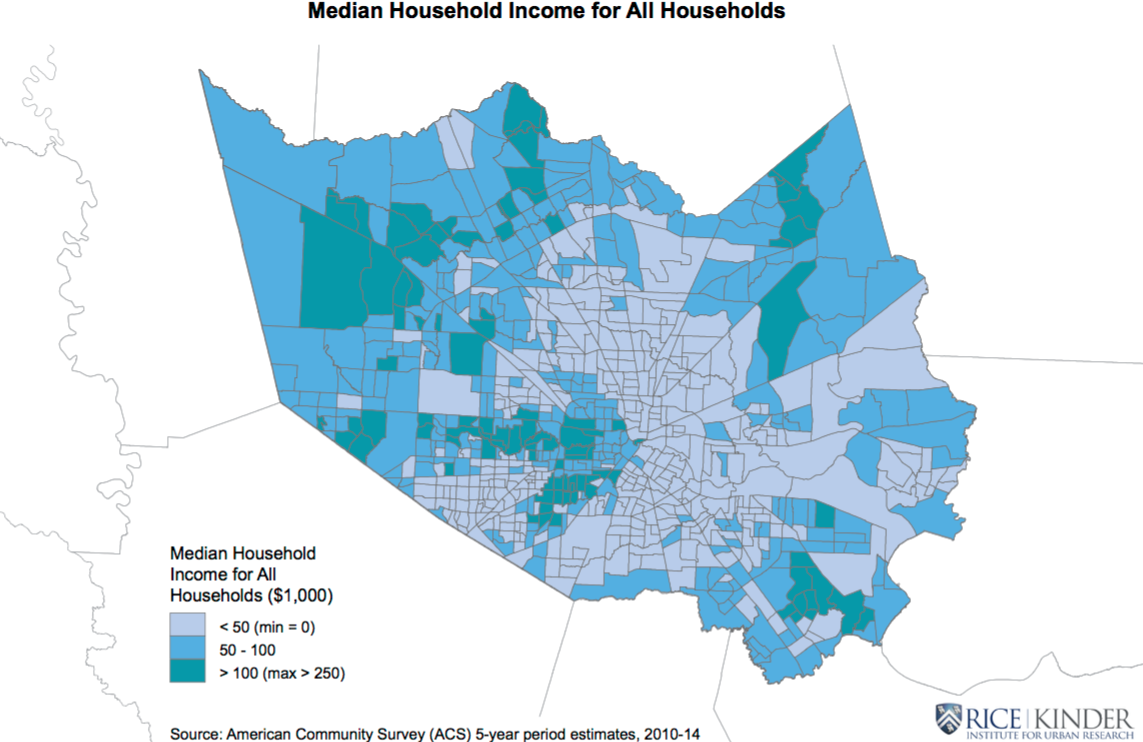
\includegraphics[width=1\linewidth]{Images/map1.png}
    \caption{Median Household Income in Houston,Texas \cite{Binkovitz_2016}}
    \label{fig:enter-label}
\end{figure}

\begin{figure}
    \centering
    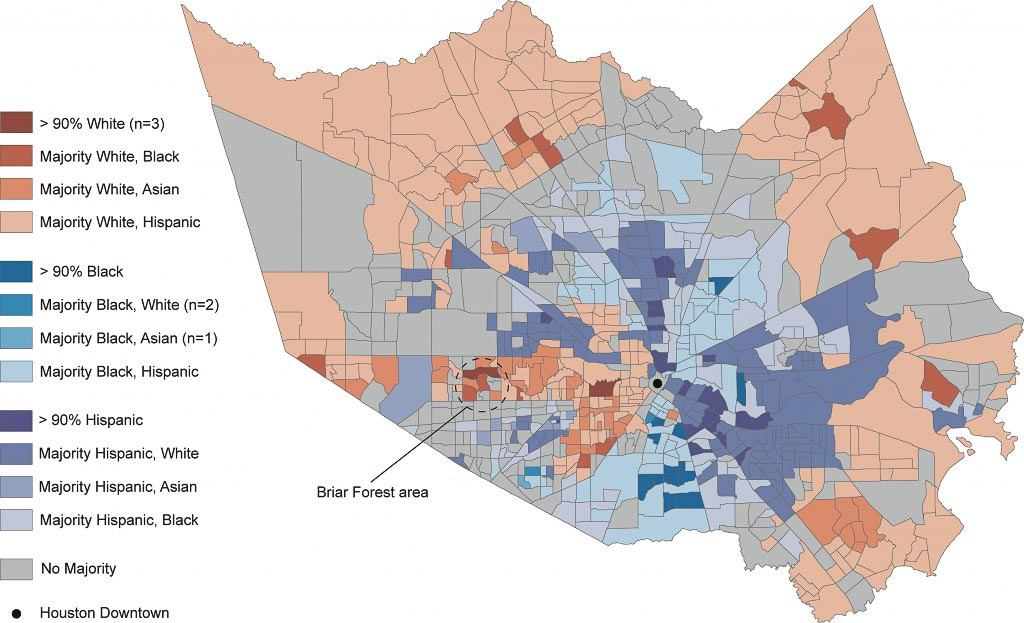
\includegraphics[width=1\linewidth]{Images/map2.jpg}
    \caption{Diversity in Houston, Texas \cite{Binkovitz_2016} }
    \label{fig:enter-label}
\end{figure}

\subsection{Method:}
In order to best observe the correlation between these factors, heat maps will be used to clearly display the correlation coefficient of each set of factors through the scale of a color bar. The correlation coefficients calculated are Pearson correlation coefficients(r) which are values that span from -1 to 1 to show how positively (r=1 means perfect positive correlation) or negatively (r=-1 means perfect negative correlation) two data sets are. Correlation coefficients are calculated via the Pearson correlation coefficient formula depicted in Fig. 3. Within each heat map, every square will represent the Pearson correlation coefficient between two factors. \par

\begin{figure}
    \begin{equation*}
    r=\frac{\sum ( x_{i} -\overline{x}) -( y_{i} -\overline{y})}{\sqrt{\sum ( x_{i} -\overline{x})^{2}\sum ( y_{i} -\overline{y})^{2}}}
    \end{equation*}
    \caption{Pearson Correlation Coefficient Formula \cite{WEBB_2021}}
    \label{fig:enter-label}
\end{figure}


\subsection{Initial Heat Map Analysis}

\begin{figure}
    \centering
    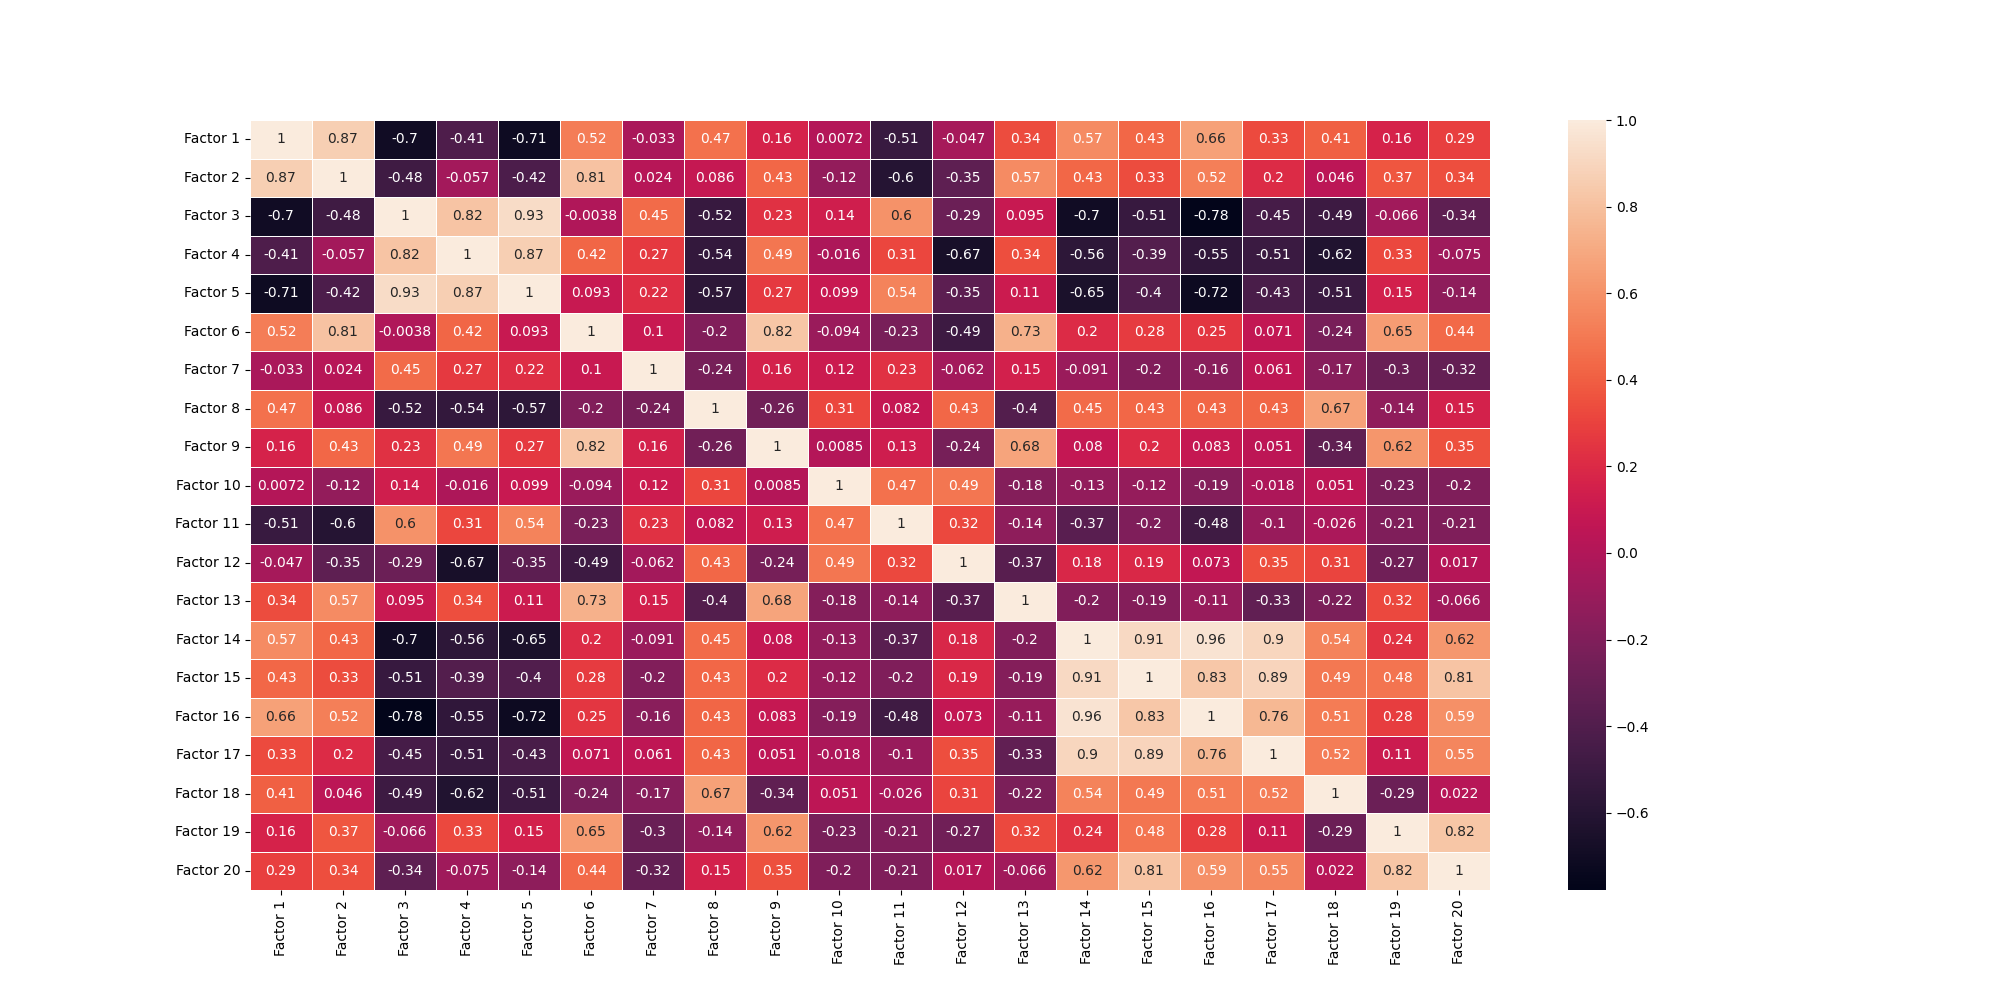
\includegraphics[width=1\linewidth]{Images/initialTotalTractHeatmap.png}
    \caption{Initial Heat map of all 15 Tracts }
    \label{fig:enter-label}
\end{figure}
\begin{figure}
    \centering
    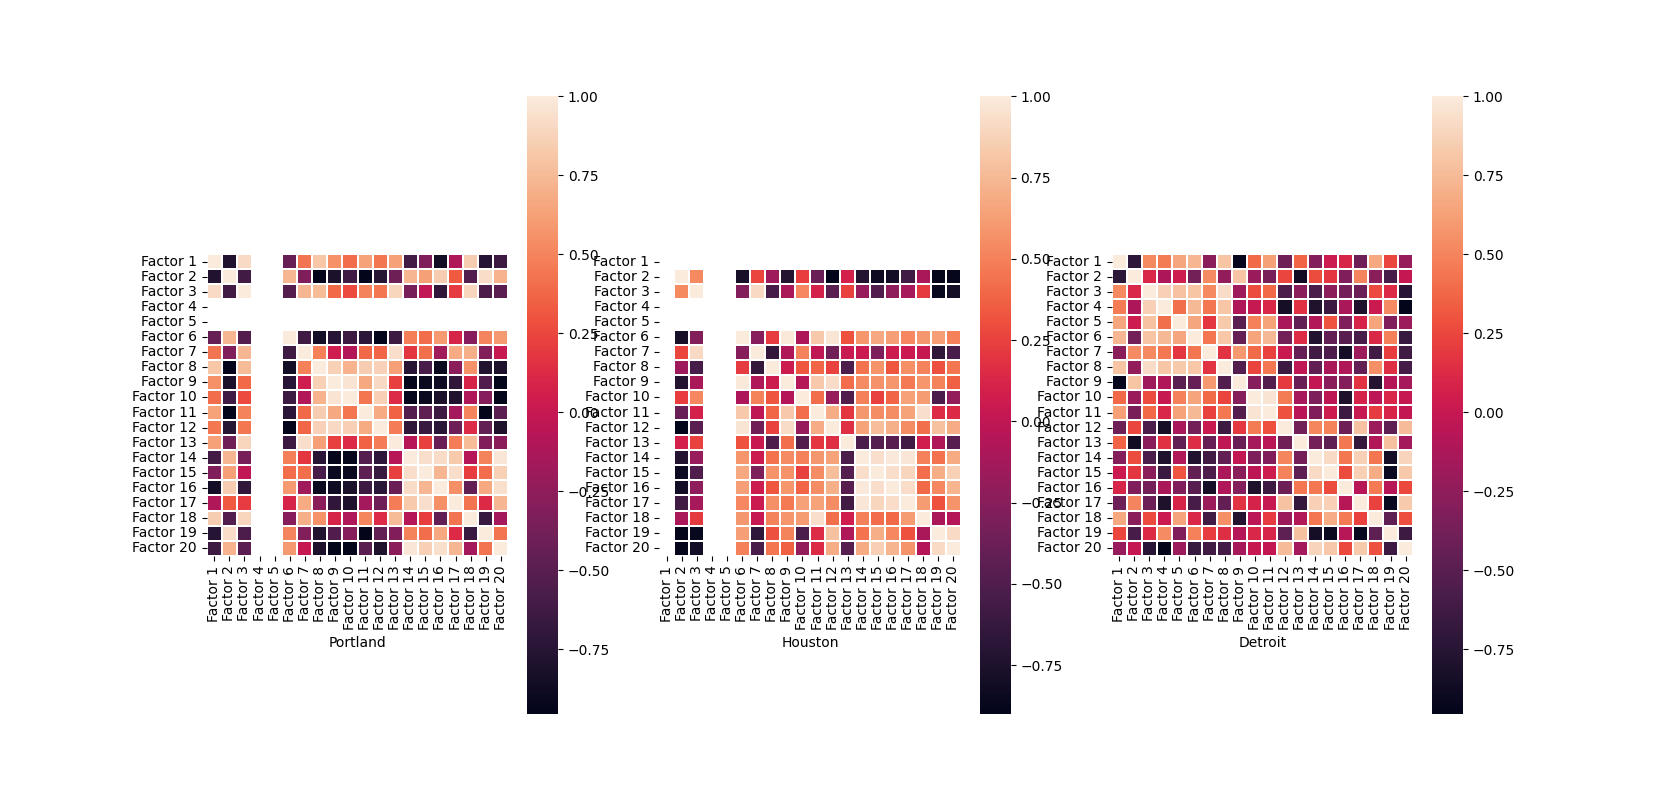
\includegraphics[width=1\linewidth]{Images/InitialTractHeatmap.png}
    \caption{Initial Heat map of 5 Tracts In Portland, Houston, And Texas }
    \label{fig:enter-label}
\end{figure}

When we examine the heat maps of Portland, Houston, and Detroit there are a few things that initially pop out. Firstly In the heat maps of Portland and Houston, there are two columns and rows that appear to be blank and show no correlation trend. What is occurring is that the correlation of those columns is not a real number because the data for those factors was the same. For the case of Portland factor 4 represents the cancer risk factor, and in the 5 tracts we examined the risk factor was always the same value. This trend also occurs in Houston and is why the columns appear blank. \par

It is also important to note that as we examine these heat maps, while much of the maps seem lightly colored and thus highly correlated, we must shift our gaze to a small section of the map. In each of these heat maps viewers should see a light-colored diagonal line of squares that represent the perfect correlation when you compare one factor to itself. Additionally, since some of the factors are environmental and some of them are demographic, it is important that we only closely examine factors from opposing categories, since it is already known that environmental factors will be correlated to one another and vice versa with demographic factors.\par

With that said it is still clear that these heat maps tell an important story. When we examine the large heat map (Fig. 4) representing all 15 tracts (5 from each city) we can see clearly that the highest correlation that we are interested in is represented between factors 1 and 2(particulate matter in the air and ozone concentration respectively), and the 7 demographic indicators. This proves our initial hypothesis that there would be a correlation due to what we know about systemic racism. With that said this is still just a very small chunk of data from the large data set EJ Screen provides us with so it is important to look at all the data together before jumping to any conclusions. \par

When we compare the Portland, Houston, and Detroit heat maps (Fig. 5), we do not necessarily see the same trends represented in the overall heat map. This variability from the overall heat map is most likely due to the very low amount of data we are analyzing. Since we are only looking at 5 tracts for each city, it is very unlikely that those 5 tracts (despite our best efforts) will be very representative of the given city, much less the state that the city resides. Therefore to get a better picture of the correlations of these factors across the US, we need to examine a much larger data set. \par




\section{Further Exploration}

\subsection{Examining all tracts together}

Fig. 6 displays the results of finding the correlation between all 20 indicators across every single tract in the United States. By compiling all of the data from throughout the United States we make our data both more reliable and less reliable at the same time. While more data points provide us with a much fuller and more representative data set, it also pulls in a lot of outliers that muddle our data. \par
Therefore looking at a heat map of the correlation within the whole United States isn't very informative, given that every state is different and thus will have different correlations. Therefore it is much more insightful to look at the correlation of these factors on a state-by-state level.\par 

Additionally, while it is interesting to look at all 20 factors compared to each other, much of this data is unnecessary and uninteresting. There is no need to compare the environmental factors to other environmental factors or the demographic factors to themselves because we are only interested in the correlation between environmental factors and their demographic counterparts. Therefore for the rest of the study, we will be zooming in on 5 main environmental factors to compare to one demographic factor: The demographic index. In doing so only the most important and insightful data will be presented. \par
\begin{figure}
    \centering
    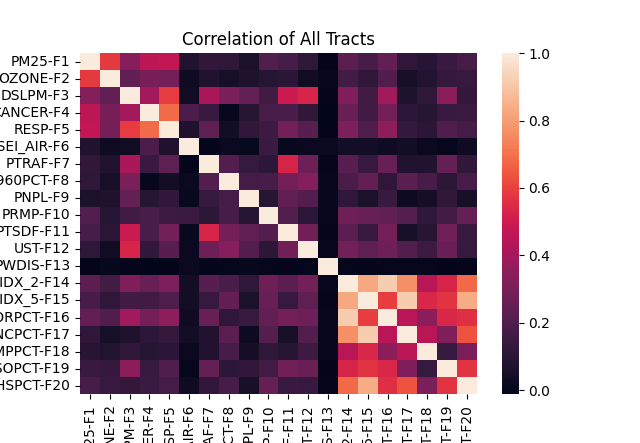
\includegraphics[width=0.5\linewidth]{Images/TotalTracts.png}
    \caption{Heat-map comparing the 20 different indicators using all of the tract data EJ Screen has}
    \label{fig:enter-label}
\end{figure}
For the remainder of the report, we will be looking at the correlation between the demographic index and 5 environmental factors: particulate matter, ozone, diesel, air toxics cancer risk, and air toxics respiratory risk index. These factors have been chosen due to their relevance in modern-day conversations surrounding climate change, and the plentiful data on them.\par

\subsection{Examining correlation on a state by state matter}

By comparing the correlation between the demographic index and these 5 different factors between the different states we produce maps that look like Fig. 7. Each state is correlated differently, some much stronger and some much weaker. Through these maps, we are able to get a much better idea of where correlation exists compared to the initial total tract heat map displayed in Fig. 6. \par
\subsection{Correlation between Demographic Index and Particulate Matter}

\begin{figure}
    \centering
    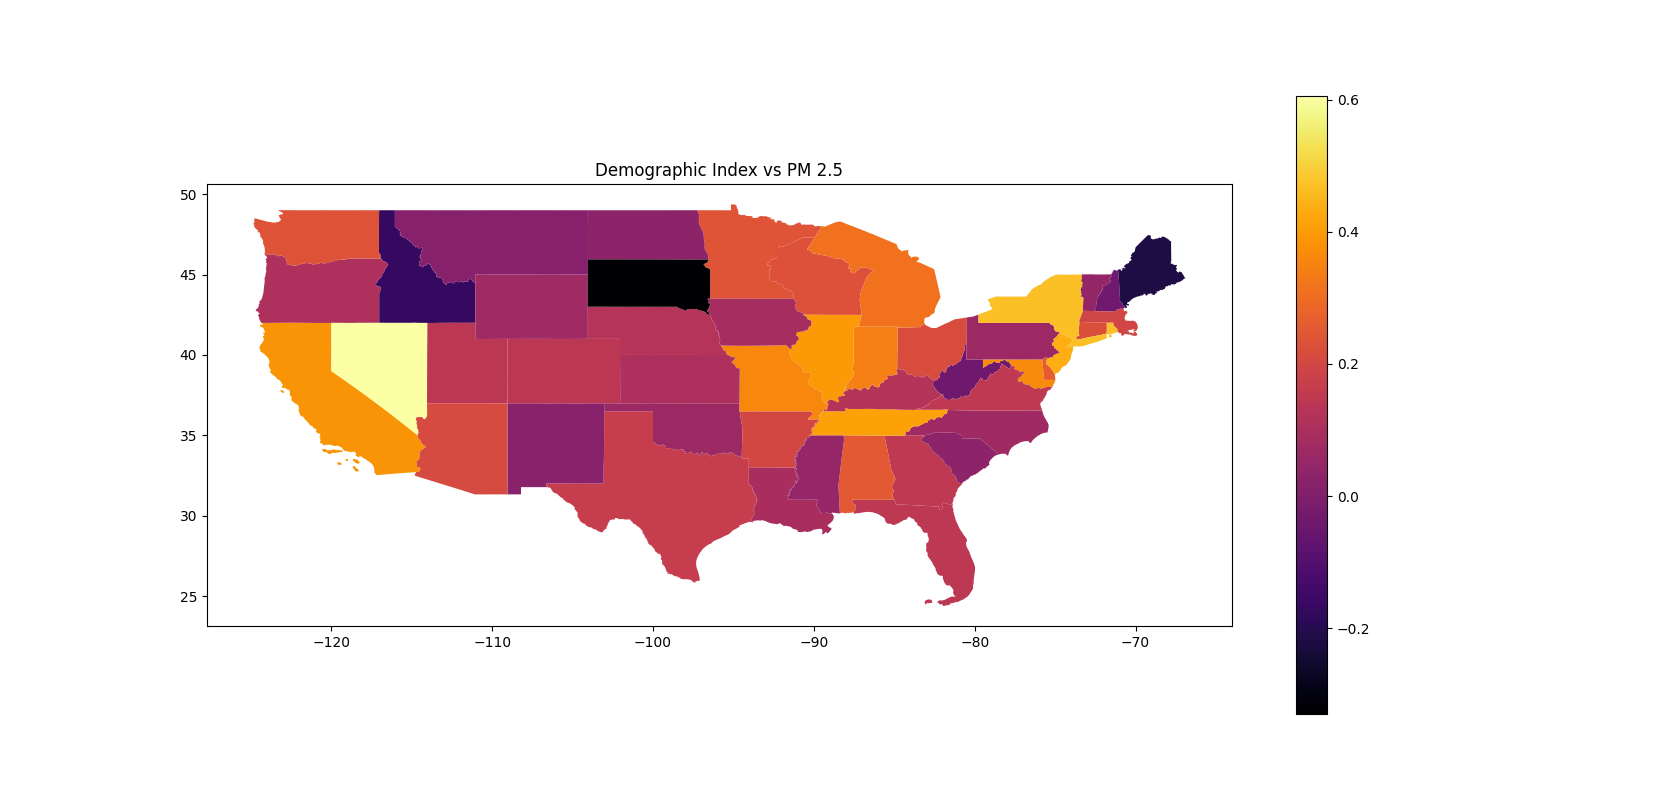
\includegraphics[width=1\linewidth]{Images/DemogrpahicIndex.VS.PM-2.5.png}
    \caption{Heat map displaying the correlation between demographic index and particulate matter(pm 2.5) across the United States}
    \label{fig:enter-label}
\end{figure}

\par
Fig. 7 displays the correlation between Demographic Index and Particulate Matter in the air between states throughout the US. The color bar allows us to quickly identify states that are on the higher end of the correlation spectrum, whether that be significantly lower correlation or higher correlation. Nevada appears to represent the highest correlation between demographic index and particulate matter within the US with a Pearson correlation coefficient of 0.605. Whereas South Dakota represents the other end of the spectrum on the map with a Pearson Correlation Coefficient of -0.329, the lowest correlation on the map. Along with Idaho and Maine whose correlation coefficients are -0.168 and -0.1765 respectively. However, what is most interesting is not the coefficients themselves but where these spikes are located on the map. Nevada and Idaho are neighbors and yet their coefficients are on opposite ends of the spectrum and the other spikes are spread across the map, which initially suggests that location has little to do with the correlation between these factors. \par
\begin{figure}
    \centering
    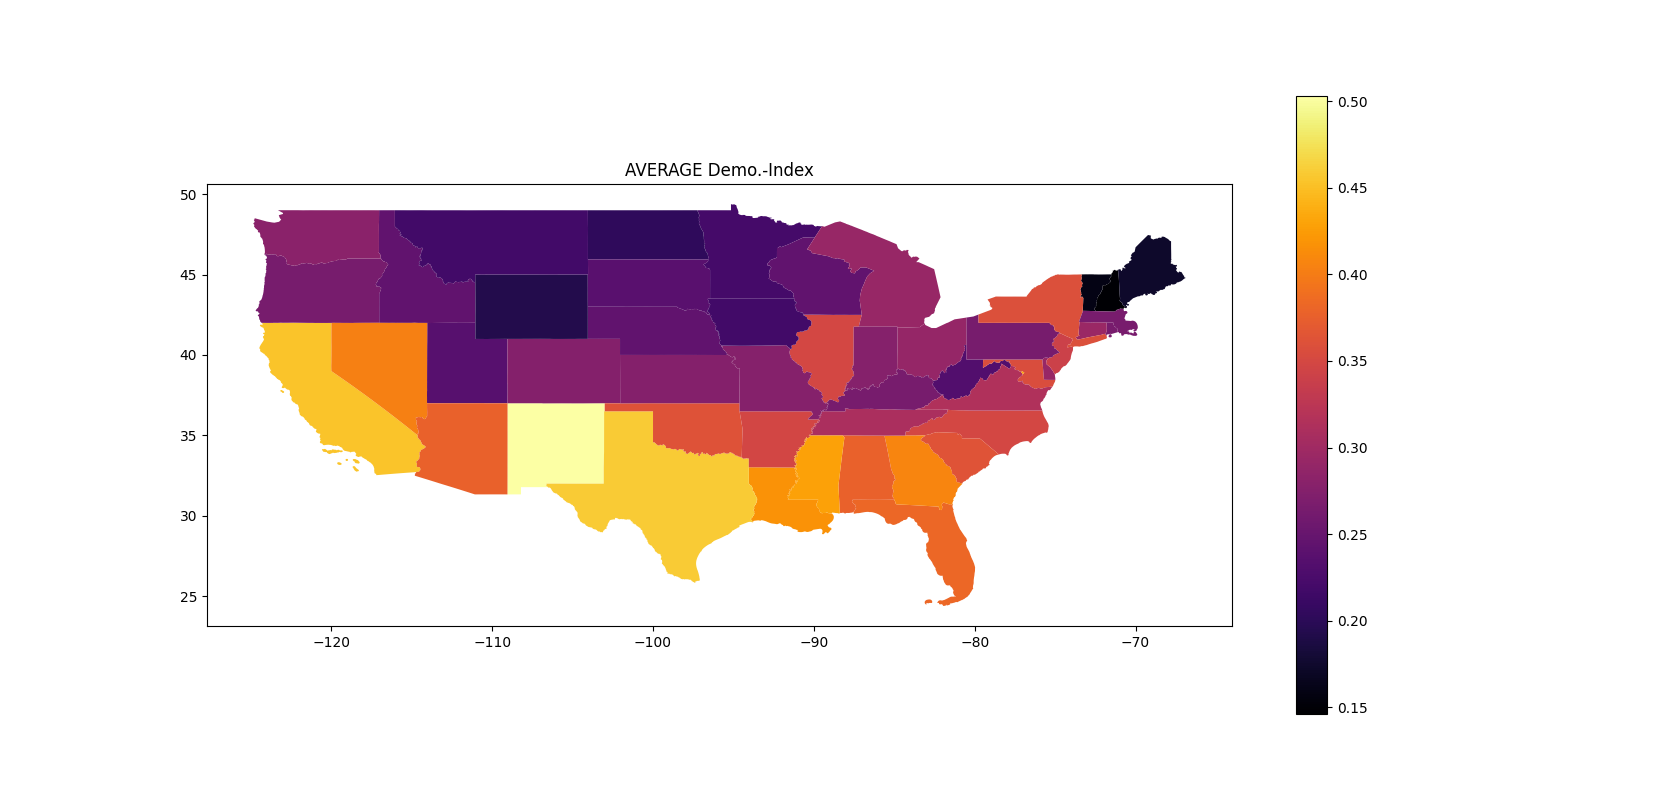
\includegraphics[width=1\linewidth]{Images/AverageDemo-Index.png}
    \caption{Average Demographic Index per State Across the US}
    \label{fig:enter-label}
\end{figure}
\begin{figure}
    \centering
    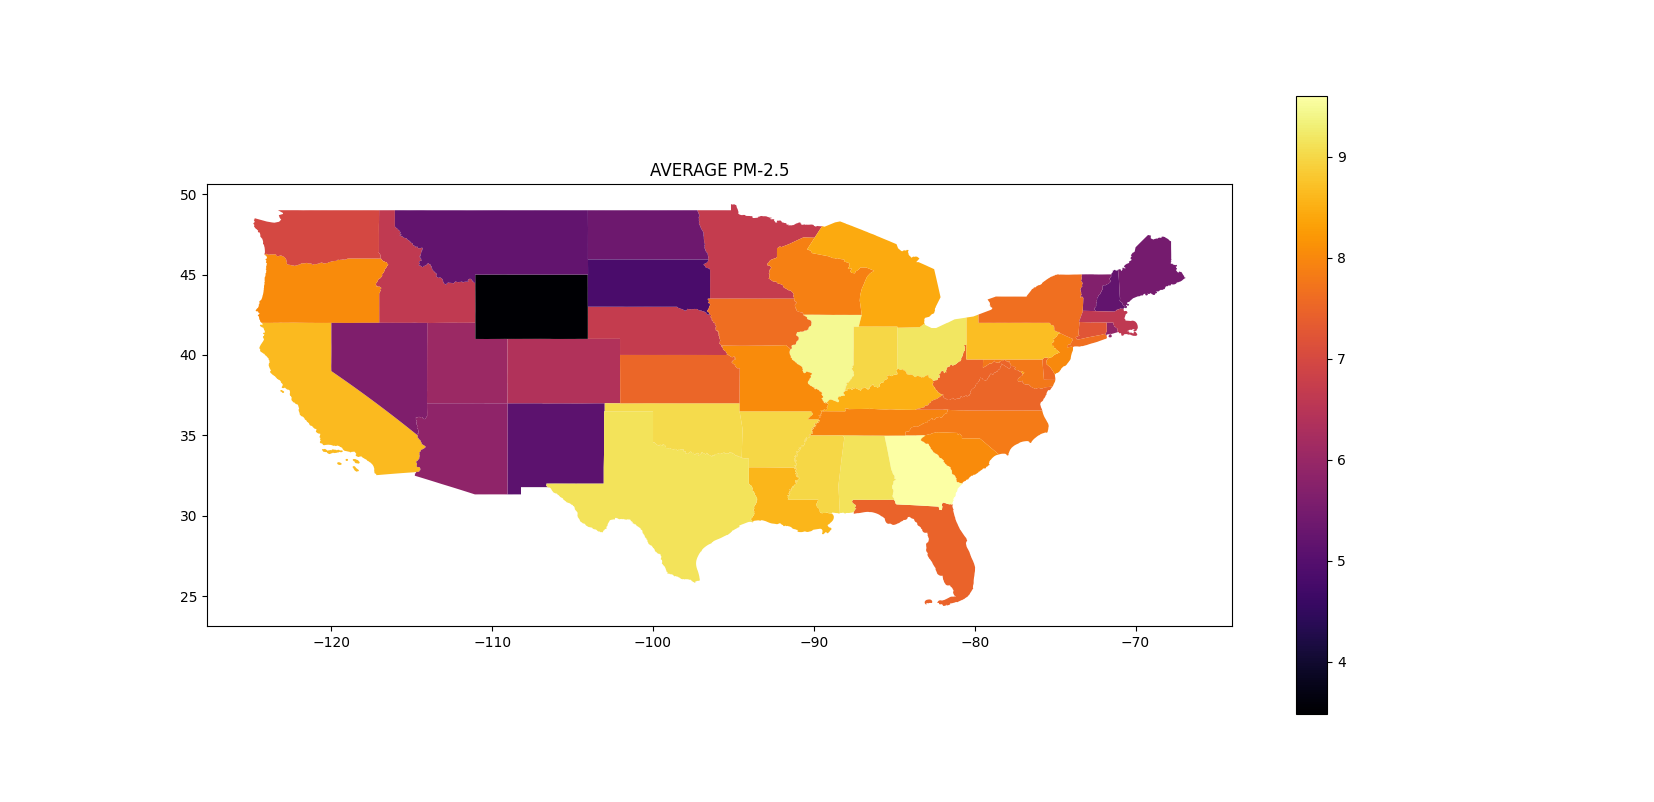
\includegraphics[width=1\linewidth]{Images/AveragePM-2.5.png}
    \caption{Average Particulate Matter in Air per State Across the US}
    \label{fig:enter-label}
\end{figure}
However, when we examine a heat map that shows the average demographic index within each state across the US(Fig. 8) the results we received become much clearer. In Fig. 8 it is clear that the Northern states are much less diverse compared to that of the Southern states with most of their demographic indexes being less than 0.3. This is problematic for the analysis of our data because if a state has a very low correlation it will be increasingly difficult to see if diversity is correlated to negative environmental effects. After all, there just isn't enough diversity within those states to have accurate data. This likely accounts for how dark/low correlated South Dakota and Maine appear to be in Fig. 7. \par
Additionally, when we examine a heat map that shows the average particulate matter in air across the US(Fig. 9) we can see that most Western and Eastern states have much higher levels of particulate matter, while the middle states have much lower levels of particulate matter. Most strikingly of which is Wyoming with the lowest level of particulate matter out of all of the states.\par
When we initially look at Fig. 7, we are both surprised, due to how scattered the high-correlated states and low-correlated states seem to be, as well as confused for the same reason. However, when we look at it alongside Fig. 8 and Fig. 9 the reasoning for results becomes much clearer. Firstly as discussed previously, the incredibly low diversity in some states such as Maine and South Dakota accounts for the extremely low correlation presented in these states in Fig. 7 However neither Fig. 8 or Fig. 9  truly account for why we see such a high correlation in Nevada in Fig. 7. Rather the answer lies in what we know about Nevada's overall population distribution and geography. Within Nevada, there are only a couple of major cities: Reno, and Las Vegas. It is within these cities that most of Nevada's population is located, otherwise, other areas of Nevada are much more sparsely populated. This likely has a large effect on our data and thus causes the correlation to appear significantly lighter compared to other states. While it is still clear correlation between the demographic index and particulate matter exists, it is likely that the distribution of the population still muddles with the data in some way.\par



\section{Conclusion}
In conclusion, it is clear that there is a correlation between an individual's demographic index and the environmental side effects they face. Through the data collected from EJ Screen, one can see the correlation between one's demographic index and a variety of factors, especially the particulate matter in the air. While the correlations are different and more striking in some states and areas compared to others, those correlations still clearly exist, and thus environmental discrimination and racism are still prominent. \par

The next step of analysis would be to zoom in on each state and compare the correlation of these factors between counties. However, due to the uneven populations of each county, and the uneven amount of tracts within different counties, there just isn't enough data to get reliable results. \par

While there are lots of different ways to continue research and analysis on this topic, the most important takeaway we can have is understanding environmental discrimination for what it is. While climate change is a pressing issue that affects every single human on earth it is clear that it effects minorities significantly more than others. Since much of the US government is made up of white privileged individuals, it is not surprising that they have done little to combat climate change since it has little physical effect on them. By understanding environmental discrimination at its core, we have the chance to change our mindset surrounding climate change by thinking not necessarily about ourselves, but about those who will be affected the most by our actions.\par


\addtolength{\textheight}{-12cm}   % This command serves to balance the column lengths
                                  % on the last page of the document manually. It shortens
                                  % the textheight of the last page by a suitable amount.
                                  % This command does not take effect until the next page
                                  % so it should come on the page before the last. Make
                                  % sure that you do not shorten the textheight too much.

%%%%%%%%%%%%%%%%%%%%%%%%%%%%%%%%%%%%%%%%%%%%%%%%%%%%%%%%%%%%%%%%%%%%%%%%%%%%%%%%



%%%%%%%%%%%%%%%%%%%%%%%%%%%%%%%%%%%%%%%%%%%%%%%%%%%%%%%%%%%%%%%%%%%%%%%%%%%%%%%%



%%%%%%%%%%%%%%%%%%%%%%%%%%%%%%%%%%%%%%%%%%%%%%%%%%%%%%%%%%%%%%%%%%%%%%%%%%%%%%%%



\section*{ACKNOWLEDGMENT}

I would like to thank Mohit Dubey for his valuable mentorship and guidance towards the execution and completion of my project.


\printbibliography
\nocite{*}

%%%%%%%%%%%%%%%%%%%%%%%%%%%%%%%%%%%%%%%%%%%%%%%%%%%%%%%%%%%%%%%%%%%%%%%%%%%%%%%%



\end{document}